\chapter{Robust Motion Planning with Global Sensitivity Optimization}\label{chap:samp}
\markboth{Robust Motion Planning with Global Sensitivity Optimization}{}% To set left/right header

% \localtableofcontents \newpage

This chapter introduces the first major contribution of this thesis, by leveraging the sensitivity concept discussed in Chapter~\ref{chap:models}.
The contribution of this chapter is twofold:
\begin{enumerate}
    \item Firstly, it addresses the generation of a desired trajectory with minimal sensitivity, ensuring that the closed-loop evolution of $\q(t)$ closely matches its nominal evolution, $\q_n(t)$. 
    While previous works have explored sensitivity optimization for generating locally sensitivity-optimal trajectories \cite{cPi,cTh}, this approach has never been applied within a global sampling-based planning framework that accounts for obstacles. 
    Therefore, the first contribution is to propose methods for efficiently performing global sensitivity-optimal motion planning.
    \item Secondly, this chapter introduces, for the first time, the use of sensitivity-based uncertainty tubes to enforce constraints in both the state and input spaces. 
    This enables the generation of intrinsically-robust motions (i.e. accounting for the controller behavior with respect to uncertainty) that ensures robustness with respect to collision avoidance with obstacles of the environment, and also with the actuation limits.
\end{enumerate}
This chapter is organized as follows: Section~\ref{sec:samp} presents a unified approach that combines robust trajectory planning with global sensitivity optimization by integrating the sensitivity computation and tube generation from Section~\ref{sec:tubes} directly into an optimal tree-based planner, such as \myglsentry{rrtstar} or \myglsentry{sst*}. 
This method enables the simultaneous generation of globally robust and sensitivity-optimal trajectories. 
The approach is evaluated on the robot models discussed in Chapter~\ref{chap:models}.
Then, Section~\ref{sec:decoupled} introduces a decoupled approach that sacrifices the global optimality of the unified method in favor of computational efficiency, demonstrating improved scalability for more complex systems while maintaining near sensitivity optimality.
Finally, some conclusions are drawn in Section~\ref{sec:concl}.

This chapter is related to the ICRA 2023 publication~\cite{cSAMP}\footnote{The results presented in this chapter slightly differ from those in the article due to improvements in implementation.}.

\section{Global robust sensitivity-optimal planning}\label{sec:samp}

This section presents how the sensitivity matrices and resulting uncertainty tube computations, outlined in Section~\ref{sec:sensi_and_tubes}, can be integrated into an asymptotically-optimal tree planner to generate robust and sensitivity-optimal trajectories. 
It introduces a unified approach that allows the planning of globally robust trajectories while simultaneously optimizing sensitivity within a single planner.

The core idea of the method is to compute the state/input sensitivity matrices (and the resulting uncertainty tubes) at each iteration of the sampling-based algorithm. 
As detailed in Section~\ref{sec:sensi_and_tubes}, these sensitivity matrices and uncertainty tubes are computed by forward-integrating a system of \myglsentry{odes} (see Equations~(\ref{eq:dyna}),~(\ref{eq:ctrl}), and~(\ref{eq:dyna_sensi})). 
Therefore, in the context of a sampling-based approach, this integration of the \myglsentry{odes} must be performed starting from a set of non-zero initial conditions (e.g., $\bPi_0$, $\q^0$, etc.), denoted $S_0$, whenever extending a node that is not the root.

The management of these initial conditions is achieved by embedding the set of final conditions (e.g., $\bPi_F$, $\q^F$, etc.), denoted $S_F$, into the node data after each extension. 
These final conditions are then reused as initial conditions for future extensions. 
It is important to note that the initial conditions of a given node are determined by the trajectory from the root node. 
Consequently, these initial conditions are specific to the parent node, making this approach applicable only in tree-based planners, where each node has exactly one parent. 
In contrast, graph-based planners, such as \myglsentry{prm}~\cite{cPRM}, cannot leverage this mechanism due to their higher degree of connectivity.
Additionally, note that, since dynamics is taken into account, the algorithms presented in this thesis utilize directed data structures (i.e., structures like directed trees that represent dependencies and directionality in motion).

This mechanism is then applied in Sections~\ref{sec:sarrt*} and~\ref{sec:sasst*} to the asymptotically optimal tree-based planners introduced in the following subsection, with the aim of developing robust, sensitivity-aware variants, commonly referred to as \gls{samp}. 
Note that, while the subsequent sections of this chapter focus on asymptotically optimal planner variants for generating globally robust sensitivity-optimal trajectories, these principles can also be easily adapted to non-asymptotically optimal planners (see Chapter~\ref{chap:sampNN}), such as the standard \gls{rrt}.

\subsection{Standard asymptotically optimal planners}\label{sec:standard_planners}

\begin{figure} [h!]
    \centering
    \includegraphics[width=0.95\linewidth]{figures/samp/rrtstar.png} 
    \caption{Illustration of the \myglsentry{rrtstar} tree extension procedure.
    The first phase (left) consists of extending the nearest node in the tree, $q^{near}$, towards a randomly sampled state, $q^{rand}$, in order to add a new collision-free state, $q^{new}$, to the tree.
    Then, an optimal connection phase is performed (middle), where the new node is optimally connected to the node with the minimum cost, $q^{min}$, from the start, within a neighborhood defined by a distance $\delta$.
    Finally, within this same neighborhood, a rewiring phase (right) is attempted to optimally reconnect the existing nodes if the cost of passing through the new state improves their current cost.}%
    \label{fig:rrtstar}%
\end{figure}

\begin{figure} [h!]
    \centering
    \includegraphics[width=0.95\linewidth]{figures/samp/sst.png} 
    \caption{Illustration of the \myglsentry{sst} tree extension procedure where green dots represent witnesses, and blue dots are current witnesses representative (i.e. the node with the best cost in the witness neighborhood) (extracted from~\cite{cSST}).
    Dynamic propagation from $x_{selected}$ generates a new node $x_{new}$, which has a better trajectory cost than its current witness representative node $x_{peer}$.
    In this case, $x_{peer}$ is pruned, and the newly propagated edge is incorporated into the tree as the new witness representative.
    If $x_{peer}$ had children with the lowest trajectory cost in their respective neighborhoods, $x_{peer}$ would remain in the tree but would no longer be considered for further propagation. 
    Inversely, if $x_{new}$ has a worse trajectory cost than $x_{peer}$, the old node $x_{peer}$ remains in the tree, and the propagation from $x_{selected}$ to $x_{new}$ is ignored.}%
    \label{fig:sst}%
\end{figure}

This subsection presents the standard asymptotically optimal sampling-based planners, which form the basis for the \myglsentry{samp} variants developed in Sections~\ref{sec:sarrt*} and~\ref{sec:sasst*}.

\paragraph{Standard RRT*}

The vanilla \gls{rrtstar}~\cite{cRRTstar} is a widely used asymptotically optimal sampling-based planner that extends the standard \gls{rrt} algorithm~\cite{cRRT} by incorporating a rewiring step to iteratively improve the quality of the trajectories in the generated tree.
It achieves this by first optimally connecting the samples to the tree and then re-evaluating the connections between sampled nodes and their neighbors based on a cost metric. 
This process ensures that the tree progressively converges toward an optimal solution as the number of samples increases.
The \myglsentry{rrtstar} tree extension process and tree rewiring phase are illustrated in Figure~\ref{fig:rrtstar}.

\paragraph{Standard SST*}

The standard \gls{sst*}~\cite{cSST} is another asymptotically optimal sampling-based planner that, unlike \myglsentry{rrtstar}, does not utilize a steering method to extend its tree but instead relies on system dynamics forward propagation.
This method grows a tree in the state space by employing Monte Carlo forward dynamic propagation to explore feasible trajectories by sampling control inputs.
To improve efficiency, \myglsentry{sst*} employs a pruning mechanism that preserves only the locally optimal solutions, thanks to a witness and representative system as illustrated in Figure~\ref{fig:sst}.
This approach ensures that the planner focuses on promising regions of the state space, reducing redundant computations while maintaining theoretical guarantees of near-optimality. 
By combining these features, \myglsentry{sst*} offers a powerful solution for kinodynamic motion planning in complex systems.

\subsection{Sensitivity-Aware RRT* (SARRT*)}\label{sec:sarrt*}

\begin{algorithm}[h!]
    \caption{SARRT$^* [q^{init}, q^{goal}]$}\label{alg:SARRT*}
    \begin{algorithmic}[1]
        \State $T \gets$ InitTree$({q^{init}, q^{goal}});$
        \While{\textbf{not} StopCondition$(T, {q^{goal}})$}  
            \State $q^{rand} \gets $Sample()$;$
            \State $q^{nearest} \gets$ Nearest$(T,{q^{rand}});$
            \State $\q_d \gets$ Steer$({q^{nearest}},{q^{rand}});$
            \State $S_0 \gets $GetNodeConditions$({q^{nearest}});$
            \State $\left \{\q_n, \u_n, \Rq, \Ru, S_F \right \}  \gets $SolveODEs$(\q_d, S_0);$
            \If {IsRobust$(\Rq,\Ru, \q_n, \u_n)$}
                \State $q^{min} \gets q^{nearest};$
                \State SetNodeConditions$({q^{rand}}, S_{F});$
                \State $Q^{near} \gets$ NearestNodes$(T,{q^{rand}});$
                \State RobustOptimalConnection$(T, Q^{near}, q^{rand}, q^{min});$
                \State RobustRewire$(T, Q^{near}, q^{min});$
            \EndIf
        \EndWhile
        \State \textbf{return} GetTrajectory$(T, q^{init}, q^{goal})$;
    \end{algorithmic}
\end{algorithm}

% For clarity in the pseudo-code, the temporal notation is omitted from this subsection. 
% Thus, bold symbols refer to trajectory vectors (e.g., $\q_d$ represents a desired trajectory, $\Rq$ stands for the uncertainty tube radii along a trajectory, etc.), while non-bold symbols represent values at a single state (e.g., $q^{rand}$ denotes a random state, and $S_0$ represents the initial conditions of the \myglsentry{odes} at a given trajectory state, etc.).

The first implementation presented in Algorithm~\ref{alg:SARRT*}\footnote{For clarity in the pseudo-code, the temporal notation is omitted from this subsection. 
Thus, bold symbols refer to trajectory vectors (e.g., $\q_d$ represents a desired trajectory, $\Rq$ stands for the uncertainty tube radii along a trajectory, etc.), while non-bold symbols represent values at a single state (e.g., $q^{rand}$ denotes a random state, and $S_0$ represents the initial conditions of the \myglsentry{odes} at a given trajectory state, etc.).} is a variant of the widely used \myglsentry{rrtstar}~\cite{cRRTstar}, denoted as \gls{sarrt*}, as a particular instance of \myglsentry{samp}.
The tree is initialized with the desired initial and goal robot states, $(q^{init}, q^{goal})$ (line 1), and the algorithm continues until a user-defined stopping condition is met (line 2).
Such a criterion can include a maximum number of iterations, a maximum runtime, a cost convergence threshold, etc.

The first stage of the algorithm follows the same standard procedure as the vanilla \myglsentry{rrtstar}, including sampling a desired robot state $q^{rand}$ and finding its nearest neighbor $q^{nearest}$ in the tree structure (lines 3 and 4, respectively) using an efficient distance metric (further discussed in Section~\ref{sec:samp_simu}).
Then, a steering method (such as the ones presented in Section~\ref{sec:kinosplines} and~\ref{sec:dubins}) is employed to generate a desired local trajectory $\q_d$ that extends $q^{nearest}$ toward $q^{rand}$.
Note that if a maximum local distance is imposed, $q^{rand}$ is adjusted accordingly.
Next, the set of \myglsentry{odes} is solved (line 7) to compute the nominal trajectory $\q_n$, the nominal control inputs $\u_n$, and the uncertainty tubes' radii $(\Rq, \Ru)$, utilizing the initial conditions $S_0$ (line 6).

A robust feasibility check is then performed along the nominal trajectory and control inputs (line 8).
This test includes a robust collision check that accounts for the robot shape expansion due to uncertainty tubes along the state trajectory, as well as a robust verification that the control inputs do not saturate (for further details see Appendix~\ref{chap:appendixA}).
Remember that this test is carried out along the nominal values, as the uncertainty tubes are valid around them, as detailed in Section~\ref{sec:tubes}.
If the extension is feasible, the new node parent is set to $q^{nearest}$, and the final conditions $S_F$ are stored within $q^{rand}$ (line 9-10).

\begin{algorithm}[h!]
    \caption{RobustOptimalConnection$[T, Q^{near}, q^{rand}, q^{min}]$}\label{alg:RobustOptimalConnect}
    \begin{algorithmic}[1]
        \State $c^{min} \gets$ Cost$(q^{rand});$
        \For {each $q^{near} \in Q^{near}$}
            \State $\q_d \gets$ Steer$(q^{near},q^{rand});$
            \State $S_0 \gets $GetNodeConditions$({q^{near}});$
            \State $\left \{\q_n, \u_n, \Rq, \Ru, S_F \right \}  \gets $SolveODEs$(\q_d, S_0);$
            \If {IsRobust$(\Rq,\Ru, \q_n, \u_n)$}
                \If {Cost$(q^{near}) + J(\q_d) < c^{min}$}
                    \State $q^{min} \gets q^{near}; c^{min} \gets$ Cost$(q^{near}) + J(\q_d);$
                    \State SetNodeConditions$({q^{rand}}, S_{F});$
                \EndIf
            \EndIf
        \EndFor
        \State AddNewNode$(T, {q^{rand}});$
        \State AddNewEdge$(T, {q^{min}}, {q^{rand}});$
    \end{algorithmic}
\end{algorithm}

Next, the newly added node is initially connected to its nearest neighbor, but this connection does not consider the total trajectory cost from the root node. 
Therefore, an optimal connection procedure is performed. 
To determine the optimal parent of $q^{rand}$, which is temporarily assigned to $q^{min}$, an additional search is conducted within a specified neighborhood $Q^{near}$ (line 11).
Such procedure, depicted in Algorithm~\ref{alg:RobustOptimalConnect}, starts by computing the cost of the unique trajectory from the root node to $q^{rand}$ (line 1).
Then, the optimal parent $q^{min}$ is set to the node in $Q^{near}$ that allows a robust extension with the minimum cost to get to $q^{rand}$ (line 2-9).
Finally, the new node is inserted in the tree with an edge connecting it to its optimal parent (line 10-11).

\begin{algorithm}[h!]
    \caption{RobustRewire$[T, Q^{near}, q^{min}]$}\label{alg:RobustRewire}
    \begin{algorithmic}[1]
        \For {each $q^{near} \in Q^{near} \backslash \{q^{min}\}$}
            \State $\q_d \gets$ Steer$(q^{rand}, q^{near});$
            \State $S_0 \gets $GetNodeConditions$({q^{rand}});$
            \State $\left \{\q_n, \u_n, \Rq, \Ru, S_F \right \}  \gets $SolveODEs$(\q_d, S_0);$
            \If {IsRobust$(\Rq,\Ru, \q_n, \u_n)$}
                \If {Cost$(q^{rand}) + J(\q_d) <$ Cost$(q^{near})$}
                    \State $q^{parent} \gets$ GetParent$(q^{near});$
                    \State RemoveEdge$(T, q^{parent}, q^{near});$
                    \State AddNewEdge$(T, q^{rand}, q^{near});$
                    \State SetNodeConditions$(q^{near}, S_{F});$
                    \State UpdateChildren$(T, q^{near});$
                \EndIf
            \EndIf
        \EndFor
    \end{algorithmic}
\end{algorithm}

Now that the optimal feasible extension is added to the tree, \myglsentry{sarrt*} checks if any optimal rewiring can be performed using Algorithm~\ref{alg:RobustRewire}.
This rewiring phase checks, for each neighbor $q^{near}$ within $Q^{near}$, whether the trajectory from the root to $q^{near}$, passing through the newly added node $q^{rand}$, can be improved (lines 1-6).
In such case, the parent of $q^{near}$ is updated accordingly, and the final \myglsentry{odes} conditions $S_F$ (e.g. final robot simulated state $\q^F$, etc.) are also modified (lines 7-10).
Note that such final conditions are reused as initial conditions in subsequent expansions.
Finally, in contrast to the standard \myglsentry{rrtstar}, each child of the newly rewired node must be rechecked for robust feasibility, as their uncertainty tubes and control inputs may have changed due to the updated trajectory resulting from the rewiring (line 11).
Note that this final operation requires re-solving the \myglsentry{odes} for each child node, as the new trajectory from the root may modify the tubes, potentially resulting in trajectories that are no longer robust.

\subsection{Sensitivity-Aware SST* (SASST*)}\label{sec:sasst*}

It is important to note that a single iteration of \myglsentry{sarrt*} presented above requires solving the set of \myglsentry{odes} multiple times which leads to a prohibitive computing time per iteration as it will be shown in Section~\ref{sec:samp_simu}.
To mitigate this, this subsection proposes a robust sensitivity-aware variant of \gls{sst*}~\cite{cSST}, denoted \gls{sasst*}, as a particular instance of \myglsentry{samp}. 

The \myglsentry{sst*} algorithm has two key features: it reduces the number of collision checks to just one per iteration, and it uses Monte Carlo propagation to sample the control input space and perform forward dynamic propagation in an open-loop manner, eliminating the need for a steering method.
However, since the system closed-loop dynamics is required for sensitivity computation rather than open-loop Monte Carlo propagation, the latter is replaced by a desired trajectory computed by a steering method and subsequently tracked by the closed-loop system.

The \myglsentry{sasst*} variant, detailed in Algorithm~\ref{alg:SASST*}, starts with planner parameters and tree initialization (line 1-4) by splitting it into two subsets: $V_{active}$ and $V_{inactive}.$
Nodes in $V_{active}$ are those with the optimal trajectory cost from the root within their local neighborhoods. 
In contrast, nodes in $V_{inactive}$, even if suboptimal in trajectory cost, are preserved in the tree to maintain connectivity, as they have children with better trajectory costs in their respective neighborhoods. 

Then, to define local neighbors, the algorithm leverages an auxiliary set of states called "witnesses," denoted as $W$ (line 5). 
Each witness $w \in W$ is associated with a single representative node in the tree, stored in the $w.rep$ field of the witness (line 6).
This representative node corresponds to the trajectory with the lowest cost from the root within a distance $\delta_s$ of the witness $w$.
Any node within the $\delta_s$-neighborhood of $w$ that have a higher trajectory cost than $w.rep$ are removed from the active set $V_{active}$.

Next, until a user-defined condition is met, the algorithm performs for N iterations:
\begin{enumerate}
    \item A best-first selection that samples a random state from the state space and finds the best node in terms of cost from the root within a distance of $\delta_{BN}$ in the active set of the tree. 
    This node, referred as $q^{selected}$, represents the state to be propagated (line 9).
    \item Then, instead of the original Monte Carlo propagation, a random state $q^{rand}$ is sampled within a maximum distance of $q^{selected}$ (line 10), analogous to sampling a control input and propagation duration in the vanilla algorithm.
    The local trajectory connecting the two state is computed (line 11) and, the set of \myglsentry{odes} is solved (line 12-13) before performing a robust feasibility check (line 14) (see Appendix~\ref{chap:appendixA}).
    \item If the local trajectory is robustly feasible, the set $W$ is utilized by the IsNodeLocallyTheBestSST procedure (line 15) to determine whether the newly sampled state $q^{rand}$ dominates the $\delta_s$-neighborhood of its nearest witness (i.e., whether $q^{rand}$ has a lower cost than the current witness of the neighborhood it belongs to). 
    The procedure then updates the witness set $W$ accordingly.
    \item Then, the sample is added to the tree (line 16-17), and the sets of active and inactive nodes are updated.
    Nodes that no longer belong to any of these sets are pruned (line 18).
\end{enumerate}

Finally, after the N iterations, if the stopping condition is not met, the hyperparameters of the algorithm are updated (line 19-21).
These parameters are responsible for the algorithm asymptotic optimality and convergence. 
The algorithm gradually reduces the radii $\delta_s$ and $\delta_{BN}$, enabling it to explore new homotopic classes over time.

Note that in this implementation the \myglsentry{odes} need to be solved only once per iteration compared to the \myglsentry{sarrt*} implementation.

\begin{algorithm}[htp]
    \caption{SASST$^* [q^{init}, q^{goal}, N_0, \delta_{BN,0}, \delta_{s,0}, \xi]$}\label{alg:SASST*}
    \begin{algorithmic}[1]
        \State $j \gets 0; N \gets N_0;$
        \State $\delta_{s} \gets \delta_{s,0}; \delta_{BN} \gets \delta_{BN,0};$
        \State $V_{active} \gets \{q^{init}, q^{goal}\}, V_{inactive} \gets \emptyset;$
        \State $T \gets$ InitTree$(V_{active}, V_{inactive});$
        \State $w_0 \gets q^{init}, w_G \gets q^{goal}, W \gets \{w_0, w_G\};$
        \State $w_0.rep \gets q^{init}, w_G.rep \gets q^{goal};$
        \While{\textbf{not} StopCondition$(T, {q^{goal}})$}  
            \For{N iterations}
                \State $\{q^{selected}, q^{rand}\} \gets $BestFirstSelectionSST$(V_{active}, \delta_{BN});$
                \State $q^{rand} \gets$ Sample$(q^{selected}, d_{max});$
                \State $\q_d \gets$ Steer$({q^{selected}},{q^{rand}});$
                \State $S_0 \gets $GetNodeConditions$({q^{selected}});$
                \State $\left \{\q_n, \u_n, \Rq, \Ru, S_F \right \}  \gets $SolveODEs$(\q_d, S_0);$
                \If {IsRobust$(\Rq,\Ru, \q_n, \u_n)$}
                    \If{IsNodeLocallyTheBestSST$(q^{rand}, W, \delta_s)$}
                        \State $V_{active} \gets V_{active} \cup \{q^{rand}\};$
                        \State AddNewEdge$(T, q^{selected}, q^{rand});$
                        \State PruneDominatedNodesSST$(q^{rand}, V_{active}, V_{inactive});$
                    \EndIf
                \EndIf
            \EndFor
            \State $\delta_s \gets \xi\delta_s; \delta_{BN}\gets\xi\delta_{BN};$
            \State $j \gets j+1;$
            \State $N \gets (1+$log $j)\xi^{-(d+1)j}N_0;$
        \EndWhile
        \State \textbf{return} GetTrajectory$(T, q^{init}, q^{goal})$;
    \end{algorithmic}
\end{algorithm}

% \section{Integrated approach}\label{sec:unified}

% This section present how the sensitivity matrices and resulting uncertainty tubes computation can be incorporated into an assymptotically-optimal tree planner in order to generate robust and sensitivity-optimal trajectories.  

% \subsection{Overview}\label{sec:general_method}

% \paragraph{Sampling-based motion planning with system dynamic}

% As shown in Section~\ref{sec:sensi_and_tubes}, the state/input sensitivity matrices (and resulting uncertainty tubes) are computed by forward integrating the set of \myglsentry{odes} (see Equation~(\ref{eq:dyna}), Equation~(\ref{eq:ctrl}), and Equation~(\ref{eq:dyna_sensi})).
% This computation is performed using the controller time step along a given desired trajectory.
% In a sampling-based framework, this computation must be performed at each new extension to compute the trajectory cost and the associated uncertainty tubes for the robust feasibility check.
% % Although the \myglsentry{odes} need to be solved at each controller time step, it is important to note that the robust feasibility check presented in Section~\ref{sec:robust_CC} can be conducted using a coarser time step.

% Furthermore, in a sampling-based context, solving the \myglsentry{odes} from a set of non-zero initial conditions (e.g. $\bPi_0$, $\q^0$ etc.), denoted $S_0$, is required when an extension is made from a node that is not the root.
% Therefore, after a feasible extension is made and the new node is added to the structure, the set of final conditions (e.g. $\bPi_F$, $\q^F$,  etc.), denoted $S_F$, must be embedded within the new node.
% These conditions are then reused as initial conditions for future extensions.
% Moreover, it is important to note that the initial conditions of a given node are determined by the trajectory from the root node. 
% As a result, these initial conditions are specific to the parent node, making them applicable only in tree-based planners, where each node has exactly one parent.
% Indeed, graph-based planners, such as \myglsentry{prm}~\cite{cPRM}, are unable to leverage such mechanisms due to their high degree of connectivity.
% Additionally, note that, since dynamics are taken into account, the algorithms presented in this thesis utilize directed data structures (i.e., structures like directed trees that represent dependencies and directionality in motion).

% This mechanism is subsequently applied in Section~\ref{sec:samp} to the tree-based planners presented in the following paragraphs.

% \paragraph{Standard RRT*}

% The vanilla \gls{rrtstar}~\cite{cRRTstar} is a widely used asymptotically optimal sampling-based planner that extends the standard \gls{rrt}~\cite{cRRT} algorithm by incorporating a rewiring step to iteratively improve the quality of the trajectories in the generated tree.
% It achieves this by first optimally connecting the samples to the tree and then re-evaluating the connections between sampled nodes and their neighbors based on a cost metric. 
% This process ensures that the tree progressively converges toward an optimal solution as the number of samples increases.
% The \myglsentry{rrtstar} tree extension process and tree rewiring phase are illustrated in Figure~\ref{fig:rrtstar}.

% \begin{figure} [htp]
%     \centering
%     \includegraphics[width=0.95\linewidth]{figures/samp/rrtstar.png} 
%     \caption{Illustration of the \myglsentry{rrtstar} tree extension procedure.
%     The first phase (left) consists of extending the nearest node in the tree, $q^{near}$, towards a randomly sampled state,$q^{rand}$, in order to add a new collision-free state, $q^{new}$, to the tree.
%     Then, an optimal connection phase is performed (middle), where the new node is optimally connected to the node with the minimum cost, $q^{min}$, from the start, within a neighborhood defined by a distance $\delta$.
%     Finally, within this same neighborhood, a rewiring phase (right) is attempted to optimally reconnect the existing nodes if the cost of passing through the new state improves their current cost.}%
%     \label{fig:rrtstar}%
% \end{figure}

% \paragraph{Standard SST*}

% The standard \gls{sst*}~\cite{cSST} is another asymptotically optimal sampling-based planner that, unlike \myglsentry{rrtstar}, does not utilize a steering method but to extend its tree but instead relies on system dynamics forward propagation.
% This method grows a tree in the state space by employing Monte Carlo forward dynamic propagation to explore feasible trajectories by sampling control inputs.
% To improve efficiency, \myglsentry{sst} employs a pruning mechanism that preserves only the locally optimal solutions, thanks to a witness and representative system as illustrated in Figure~\ref{fig:sst}.
% This approach ensures that the planner focuses on promising regions of the state space, reducing redundant computations while maintaining theoretical guarantees of near-optimality. 
% By combining these features, \myglsentry{sst} offers a powerful solution for kinodynamic motion planning in complex systems.

% \begin{figure} [htp]
%     \centering
%     \includegraphics[width=0.95\linewidth]{figures/samp/sst.png} 
%     \caption{Illustration of the \myglsentry{sst} tree extension procedure where green dots represent witnesses, and blue dots are current witnesses representative (i.e. the node with the best cost in the witness neighborhood) (extracted from~\cite{cSST}).
%     Dynamic propagation from $x_{selected}$ generates a new node $x_{new}$, which has a better trajectory cost than its current witness representative node $x_{peer}$.
%     In this case, $x_{peer}$ is pruned, and the newly propagated edge is incorporated into the tree as the new witness representative.
%     If $x_{peer}$ had children with the lowest trajectory cost in their respective neighborhoods, $x_{peer}$ would remain in the tree but would no longer be considered for further propagation. 
%     Inversely, if $x_{new}$ has a worse trajectory cost than $x_{peer}$, the old node $x_{peer}$ remains in the tree, and the propagation from $x_{selected}$ to $x_{new}$ is ignored.}%
%     \label{fig:sst}%
% \end{figure}

% \subsection{Sensitivity-Aware Motion Planner (SAMP)}\label{sec:samp}

% The following subsection describes how the concepts outlined above can be incorporated into different tree planners to develop robust, sensitivity-aware variants, generally referred to as \gls{samp}.
% Note that although the following sections of this chapter focus on asymptotically-optimal planner variants to generate globally sensitivity-optimal trajectories, the same principles can easily be applied to non-asymptotically optimal planners (see Chapter~\ref{chap:sampNN}), such as the standard \gls{rrt}.

% For clarity in the pseudo-code, the temporal notation is omitted in this subsection. 
% Thus, bold symbols refer to time-dependent vectors (e.g., $\q_d$ represents a desired trajectory, $\Rq$ stands for the uncertainty tube radii along a trajectory, etc.), while non-bold symbols represent instantaneous vectors (e.g., $q^{rand}$ denotes a random state, and $S_0$ represents the initial conditions of the \myglsentry{odes} at a given state vector, etc.).

% \subsubsection{Sensitivity-Aware RRT* (SARRT*)}

% \begin{algorithm}[htp]
%     \caption{SARRT$^* [q^{init}, q^{goal}]$}\label{alg:SARRT*}
%     \begin{algorithmic}[1]
%         \State $T \gets$ InitTree$({q^{init}, q^{goal}});$
%         \While{\textbf{not} StopCondition$(T, {q^{goal}})$}  
%             \State $q^{rand} \gets $Sample()$;$
%             \State $q^{nearest} \gets$ Nearest$(T,{q^{rand}});$
%             \State $\q_d \gets$ Steer$({q^{nearest}},{q^{rand}});$
%             \State $S_0 \gets $GetNodeConditions$({q^{nearest}});$
%             \State $\left \{\q_n, \u_n, \Rq, \Ru, S_F \right \}  \gets $SolveODEs$(\q_d, S_0);$
%             \If {IsRobust$(\Rq,\Ru, \q_n, \u_n)$}
%                 \State $q^{min} \gets q^{nearest};$
%                 \State SetNodeConditions$({q^{rand}}, S_{F});$
%                 \State $Q^{near} \gets$ NearestNodes$(T,{q^{rand}});$
%                 \State RobustOptimalConnection$(T, Q^{near}, q^{rand}, q^{min});$
%                 \State RobustRewire$(T, Q^{near}, q^{min});$
%             \EndIf
%         \EndWhile
%         \State \textbf{return} GetTrajectory$(T, q^{init}, q^{goal})$;
%     \end{algorithmic}
% \end{algorithm}

% \begin{algorithm}[htp]
%     \caption{RobustOptimalConnection$[T, Q^{near}, q^{rand}, q^{min}]$}\label{alg:RobustOptimalConnect}
%     \begin{algorithmic}[1]
%         \State $c^{min} \gets$ Cost$(q^{rand});$
%         \For {each $q^{near} \in Q^{near}$}
%             \State $\q_d \gets$ Steer$(q^{near},q^{rand});$
%             \State $S_0 \gets $GetNodeConditions$({q^{near}});$
%             \State $\left \{\q_n, \u_n, \Rq, \Ru, S_F \right \}  \gets $SolveODEs$(\q_d, S_0);$
%             \If {IsRobust$(\Rq,\Ru, \q_n, \u_n)$}
%                 \If {Cost$(q^{near}) + J(\q_d) < c^{min}$}
%                     \State $q^{min} \gets q^{near}; c^{min} \gets$ Cost$(q^{near}) + J(\q_d);$
%                     \State SetNodeConditions$({q^{rand}}, S_{F});$
%                 \EndIf
%             \EndIf
%         \EndFor
%         \State AddNewNode$(T, {q^{rand}});$
%         \State AddNewEdge$(T, {q^{min}}, {q^{rand}});$
%     \end{algorithmic}
% \end{algorithm}

% \begin{algorithm}[htp]
%     \caption{RobustRewire$[T, Q^{near}, q^{min}]$}\label{alg:RobustRewire}
%     \begin{algorithmic}[1]
%         \For {each $q^{near} \in Q^{near} \backslash \{q^{min}\}$}
%             \State $\q_d \gets$ Steer$(q^{rand}, q^{near});$
%             \State $S_0 \gets $GetNodeConditions$({q^{rand}});$
%             \State $\left \{\q_n, \u_n, \Rq, \Ru, S_F \right \}  \gets $SolveODEs$(\q_d, S_0);$
%             \If {IsRobust$(\Rq,\Ru, \q_n, \u_n)$}
%                 \If {Cost$(q^{rand}) + J(\q_d) <$ Cost$(q^{near})$}
%                     \State $q^{parent} \gets$ GetParent$(q^{near});$
%                     \State RemoveEdge$(T, q^{parent}, q^{near});$
%                     \State AddNewEdge$(T, q^{rand}, q^{near});$
%                     \State SetNodeConditions$(q^{near}, S_{F});$
%                     \State UpdateChildren$(T, q^{near});$
%                 \EndIf
%             \EndIf
%         \EndFor
%     \end{algorithmic}
% \end{algorithm}

% The first implementation presented in Algorithm~\ref{alg:SARRT*} is a variant of the widely used \myglsentry{rrtstar}~\cite{cRRTstar}, denoted \gls{sarrt*} as a particular instance of \myglsentry{samp}.
% The tree is initialized with the desired initial and goal robot states, $(q^{init}, q^{goal})$ (line 1), and the algorithm continues until a user-defined stopping criterion is met (line 2).
% Such a criterion can include a maximum number of iterations, a maximum runtime, a cost convergence threshold, etc.

% The first stage of the algorithm follows the same standard procedure as the vanilla \myglsentry{rrtstar}, including sampling a desired robot state $q^{rand}$ and finding its nearest neighbor $q^{nearest}$ in the tree structure (lines 3 and 4, respectively) using an efficient distance metric (further discussed in Section~\ref{sec:samp_simu}).
% Then, a steering method (such as the ones presented in Section~\ref{sec:kinosplines} and~\ref{sec:dubins}) is employed to generate a desired local trajectory $\q_d$ that extends $q^{nearest}$ toward $q^{rand}$.
% Note that if a maximum local distance is imposed, $q^{rand}$ is adjusted accordingly.
% Next, the set of \myglsentry{odes} is solved (line 7) to compute the nominal trajectory $\q_n$, the nominal control inputs $\u_n$, and the uncertainty tubes $(\Rq, \Ru)$, utilizing the initial conditions $S_0$ (line 6).

% A robust feasibility check is then performed along the nominal trajectory and control inputs (line 8).
% This test includes a robust collision check that accounts for the robot shape expansion due to uncertainty tubes along the state trajectory, as well as a robust verification that the control inputs do not saturate (for further details see Appendix~\ref{chap:appendixA}).
% Remember that this test is carried out along the nominal values, as the uncertainty tubes are valid around them, as detailed in Section~\ref{sec:tubes}.
% If the extension is feasible, the new node parent is temporarily set to $q^{nearest}$, and the final conditions $S_F$ are temporarily stored within $q^{rand}$ (line 9-10).

% Next, to identify the optimal parent of $q^{rand}$, which is temporarily assigned to $q^{min}$, an additional search is conducted within a specified neighborhood $Q^{near}$ (line 11).
% Such procedure, depicted in Algorithm~\ref{alg:RobustOptimalConnect}, starts by computing the cost of the unique trajectory from the root node to $q^{rand}$ (line 1).
% Then, the optimal parent $q^{min}$ is set to the node in $Q^{near}$ that allows a robust extension with the minimum cost to get to $q^{rand}$ (line 2-9).
% Finally, the new node is inserted in the tree with an edge connecting it to its optimal parent (line 10-11).

% Now that the optimal feasible extension is added to the tree, the \myglsentry{sarrt*} checks if any optimal rewiring can be performed using Algorithm~\ref{alg:RobustRewire}.
% This rewiring phase checks, for each neighbor $q^{near}$ within $Q^{near}$, whether the trajectory from the root to $q^{near}$, passing through the newly added node $q^{rand}$, can be improved (lines 1-6).
% In such case, the parent of $q^{near}$ is updated accordingly, and the final \myglsentry{odes} conditions ($S_F$) are also modified (lines 7-10).
% Note that such final conditions are reused as initial conditions in subsequent expansions.
% Finally, in contrast to the standard \myglsentry{rrtstar}, each child of the newly rewired node must be rechecked for robust feasibility, as their uncertainty tubes and control inputs may have changed due to the updated trajectory resulting from the rewiring (line 11).
% Note that this final operation requires re-solving the \myglsentry{odes} for each child node.

% \subsubsection{Sensitivity-Aware SST* (SASST*)}

% It is important to note that a single iteration of \myglsentry{sarrt*} presented above requires solving the set of \myglsentry{odes} multiple times which leads to a prohibitive computation time per iteration as shown in Section~\ref{sec:samp_simu}.
% To mitigate this impact, this subsection proposes a robust sensitivity-aware variant of the \gls{sst*}~\cite{cSST}, denoted \gls{sasst*} as a particular instance of \myglsentry{samp}. 

% The \myglsentry{sst*} algorithm has two key features: it reduces the number of collision checks to just one per iteration and uses Monte Carlo propagation to sample the control input space and perform forward dynamic propagation, eliminating the need for a steering method.
% However, since the system closed-loop dynamics is used for sensitivity computation rather than open-loop Monte Carlo propagation, the latter is replaced by a desired trajectory computed by a steering method.

% The \myglsentry{sasst*} variant, detailed in Algorithm~\ref{alg:SASST*}, starts with metrics and tree initialization (line 1-4) by splitting it into two subsets: $V_{active}$ and $V_{inactive}.$
% Nodes in $V_{active}$ are those with the optimal trajectory cost from the root within their local neighborhoods. 
% In contrast, nodes in $V_{inactive}$ while suboptimal in trajectory cost, are preserved in the tree to maintain connectivity, as they have children with better trajectory costs in their respective neighborhoods. 

% Then, to define local neighborhoods, the algorithm leverages an auxiliary set of states called "witnesses," denoted as $W$ (line 5). 
% Each witness $w \in W$ is associated with a single representative node in the tree, stored in the $w.rep$ field of the witness (line 6).
% This representative node corresponds to the trajectory with the lowest cost from the root within a distance $\delta_s$ of the witness $w$.
% Any nodes within the $\delta_s$-neighborhood of $w$ that have a higher trajectory cost than $w.rep$ are removed from the active set $V_{active}$.

% Next, until a user defined criterion is met, the algorithm performs for N iterations:
% \begin{enumerate}
%     \item A best-first selection that samples a random state from the state space and finds the best node in terms of cost from the root within a distance of $\delta_{BN}$ in the active set of the tree. 
%     This node, referred as $q^{selected}$, represents the state to be propagated (line 9).
%     \item Then, instead of the original Monte Carlo propagation, a random state $q^{rand}$ is sampled within a maximum distance of $q^{selected}$ (line 10), analogous to sampling a control input and propagation duration in the vanilla algorithm.
%     The local trajectory connecting the two state is computed (line 11) and, as discussed in Section~\ref{sec:general_method}, the set of \myglsentry{odes} is solved (line 12-13) before performing a robust feasibility check (line 14) (see Appendix~\ref{chap:appendixA}).
%     \item If the local trajectory is robustly feasible, the set $W$ is used by the IsNodeLocallyTheBestSST procedure (line 15) to check whether the newly sampled state $q^{rand}$ dominates the $\delta_s$-neighborhood of its closest witness and to update the witness set $W$ accordingly.
%     \item Then, the sample is added to the tree (line 16-17), and the sets of active and inactive nodes are updated.
%     Nodes that no longer belong to any of these sets are pruned (line 18).
% \end{enumerate}

% Finally, after the N iterations, if the stopping criterion is not met, the hyperparameters of the algorithm are updated (line 19-21).
% These parameters are responsible for the algorithm asymptotic optimality and convergence. 
% The algorithm gradually reduces the radii $\delta_s$ and $\delta_{BN}$, enabling it to explore new homotopic classes over time.

% Note that in this implementation the \myglsentry{odes} need to be solved only once per iteration compared to the \myglsentry{sarrt*} implementation.

% \begin{algorithm}[htp]
%     \caption{SASST$^* [q^{init}, q^{goal}, N_0, \delta_{BN,0}, \delta_{s,0}, \xi]$}\label{alg:SASST*}
%     \begin{algorithmic}[1]
%         \State $j \gets 0; N \gets N_0;$
%         \State $\delta_{s} \gets \delta_{s,0}; \delta_{BN} \gets \delta_{BN,0};$
%         \State $V_{active} \gets \{q^{init}, q^{goal}\}, V_{inactive} \gets \emptyset;$
%         \State $T \gets$ InitTree$(V_{active}, V_{inactive});$
%         \State $w_0 \gets q^{init}, w_G \gets q^{goal}, W \gets \{w_0, w_G\};$
%         \State $w_0.rep \gets q^{init}, w_G.rep \gets q^{goal};$
%         \While{\textbf{not} StopCondition$(T, {q^{goal}})$}  
%             \For{N iterations}
%                 \State $\{q^{selected}, q^{rand}\} \gets $BestFirstSelectionSST$(V_{active}, \delta_{BN});$
%                 \State $q^{rand} \gets$ Sample$(q^{selected}, d_{max});$
%                 \State $\q_d \gets$ Steer$({q^{selected}},{q^{rand}});$
%                 \State $S_0 \gets $GetNodeConditions$({q^{selected}});$
%                 \State $\left \{\q_n, \u_n, \Rq, \Ru, S_F \right \}  \gets $SolveODEs$(\q_d, S_0);$
%                 \If {IsRobust$(\Rq,\Ru, \q_n, \u_n)$}
%                     \If{IsNodeLocallyTheBestSST$(q^{rand}, W, \delta_s)$}
%                         \State $V_{active} \gets V_{active} \cup \{q^{rand}\};$
%                         \State AddNewEdge$(T, q^{selected}, q^{rand});$
%                         \State PruneDominatedNodesSST$(q^{rand}, V_{active}, V_{inactive});$
%                     \EndIf
%                 \EndIf
%             \EndFor
%             \State $\delta_s \gets \xi\delta_s; \delta_{BN}\gets\xi\delta_{BN};$
%             \State $j \gets j+1;$
%             \State $N \gets (1+$log $j)\xi^{-(d+1)j}N_0;$
%         \EndWhile
%         \State \textbf{return} GetTrajectory$(T, q^{init}, q^{goal})$;
%     \end{algorithmic}
% \end{algorithm}

\subsection{Cost function}\label{sec:sensi_cost}

While the previously mentioned \myglsentry{samp} variants are sensitivity-aware in the sense that they leverage sensitivity-based uncertainty tubes, they can be applied to optimize various non sensitivity-based cost functions, such as length or obstacle clearance.
However, as stated earlier, the goal is to generate robust and sensitivity-optimal trajectories.
To achieve this, the first step is to define an appropriate sensitivity-based cost function.
The approaches in~\cite{cPi, cTh} proposed leveraging the Frobenius norm of the sensitivity matrices (Equation~\ref{eq:sensi}).
However, this formulation does not exploit the available information on the uncertainty ranges, $\delta \p$, and the subsequent uncertainty tubes.

Therefore, it is preferable to consider the largest eigenvalue of the kernel matrix $\bPi(t) \W \bPi(t)^T$ as \emph{sensitivity norm}, since this represents the largest (worst-case) deviation in the state space. 
In particular, letting $\lambda_i(t)$ be the eigenvalues of $\bPi(t) \W \bPi(t)^T$, a smooth approximation of the $\max(\cdot)$ operator is performed with the $p$-norm:
\begin{equation}
    \lambda_{max}(t)\approx \left(\sum \lambda_{i}(t)^p\right)^{1/p}.
\end{equation} 

However, such function is neither additive (i.e., considering two desired trajectories ($\q_{d,1}(t), \q_{d,2}(t)$), the cost of their concatenation $c(\q_{d,1}(t)|\q_{d,2}(t)) \neq c(\q_{d,1}(t)) + c(\q_{d,2}(t))$), nor monotonic as depicted in Figure~\ref{fig:monotonic}.
Therefore, it is unsuitable for global optimization using sampling-based motion planners like~\cite{cRRTstar, cSST}, since they require additive and monotonic objective functions.
The total cost function $c(\q_d(t))$ for a desired trajectory $\q_d(t)$ is then defined considering its integral along the desired trajectory s.t.:
\begin{equation} \label{eq:cost_function}
    c(\q_d(t))=\int_{t_{0}}^{t_{f}}\lambda_{max}(\tau)d\tau.
\end{equation}
Minimization of this cost will smooth deviation of the state tube along the whole motion.

\begin{figure} [htp]
    \centering
    \subfloat[\centering p-norm]{{\includegraphics[width=0.45\linewidth]{figures/samp/non_monotoic.png} }}% 
    \subfloat[\centering Integrated p-norm]{{\includegraphics[width=0.45\linewidth]{figures/samp/integrated_monotoic.png} }}%
    \caption{Non monotonic p-norm (a) and its integration (b) along a 70-state trajectory for a quadrotor example.}%
    \label{fig:monotonic}%
\end{figure}

\subsection{Simulation results}\label{sec:samp_simu}

This subsection presents the results of trajectory planning using the previously discussed variants, evaluated based on computing time and robustness for the two systems (quadrotor and differential drive robots) introduced in Chapter~\ref{chap:models}.
To assess the impact of planning robust, globally sensitivity-optimal trajectories, both \myglsentry{sarrt*} and \myglsentry{sasst*} are compared with their respective non-robust vanilla versions, which focus on optimizing trajectory length.
The objective is to verify the ability of the proposed variants to generate robust solutions, and to evaluate the computational overhead of solving the huge number\footnote{From few thousands for non asymptotically optimal planners, up to a hundred of thousands for asymptotically optimal planners.} of \myglsentry{odes} during the random-trees expansions until an asymptotically optimal solution is found.
Results are obtained from the implementations of the planners within the \gls{ompl}~\cite{cOMPL}, and collision detection is performed using the widely used C implementation of PyBullet~\cite{cBullet}.
The \myglsentry{odes} are solved using the JiTCODE~\cite{cJit} module which converts the equations to be integrated into C-compiled code.
The Euler integrator is then used to solve each ODE and take advantage of this compiled function.
Although the Euler method is less accurate than a Runge-Kutta 4-based method (e.g., dopri5), it is chosen because the uncertainty tubes are already based on a first-order approximation (see Section~\ref{sec:tubes}), and faster computational efficiency are preferred over higher accuracy in this context.

\subsubsection{Differential drive robot}\label{sec:unic_setup_samp}

\paragraph{Robot setup}

This subsection presents results for the differential drive robot model depicted in Section~\ref{sec:unic_model}, with the following set of uncertain parameters $\p = [r, \, d]^T \in \mathbb{R}^{2}$, where $d$ is the length between the two wheels, and $r$ is the wheel radius.
The nominal value vector is set to $\p_n = [0.1m, \, 0.4m]^T$, with an associated uncertainty range of $\delta\p = [3\%, \, 3\%]^T$, representing the percentage deviation from their corresponding nominal values.
Therefore, in this differential drive robot application, $\bPi \in \mathbb{R}^{3\times2}$, $\bPixi\in \mathbb{R}^{3\times2}$, and $\bTheta \in \mathbb{R}^{2\times2}$.
As a result, the computations necessary to find the uncertainty tubes involve solving 16 \myglsentry{odes}.
The uncertainty tubes considered for this application are defined as $\Rq = [r_x, \, r_y]^T \in \mathbb{R}^2$, representing the uncertainty tubes along the x,y-axes of the state respectively, and $\Ru = [r_{u1}, \, r_{u2}]^T \in \mathbb{R}^2$, representing the uncertainty tubes along the two control input space axes ($\omega_r$ and $\omega_l$).
The controller gains are set to $\k_c = [1.5, \, 8.0, \, 0.2]^T$, and the control input limits are set to $\u_{max} = [60, \, 60]^T$, corresponding to the maximum speed of the two wheels expressed in rad/s.

\paragraph{Planning setup}

Remind that the local planning method used is the Dubins curves (see Section~\ref{sec:dubins}) with $v_{magn}$ = 1.0 m/s. 
Using the true cost-to-go from Equation~(\ref{eq:cost_function}) as the distance metric is known to be computationally expensive. 
Since this cost is closely tied to the trajectory length via the integral term, the length of the Dubins curves is employed as the distance metric to define the sample neighborhood. 
However, within this neighborhood, the cost from Equation~(\ref{eq:cost_function}) is used as the true cost-to-go.

The hyperparameters for \myglsentry{sasst*} are selected based on the recommendations in~\cite{cSST} for a differential drive robot, with the following values: $N_0 = 10000$, $\delta_s = 0.5$, $\delta_{BN} = 1$, and $\xi = 0.9$.
For the maximum local distance, $d_{max}$ is set to 1.0.

\begin{figure} [h!]
    \centering
    \subfloat[\centering Maximum local distance based on space size in \myglsentry{rrtstar}]{{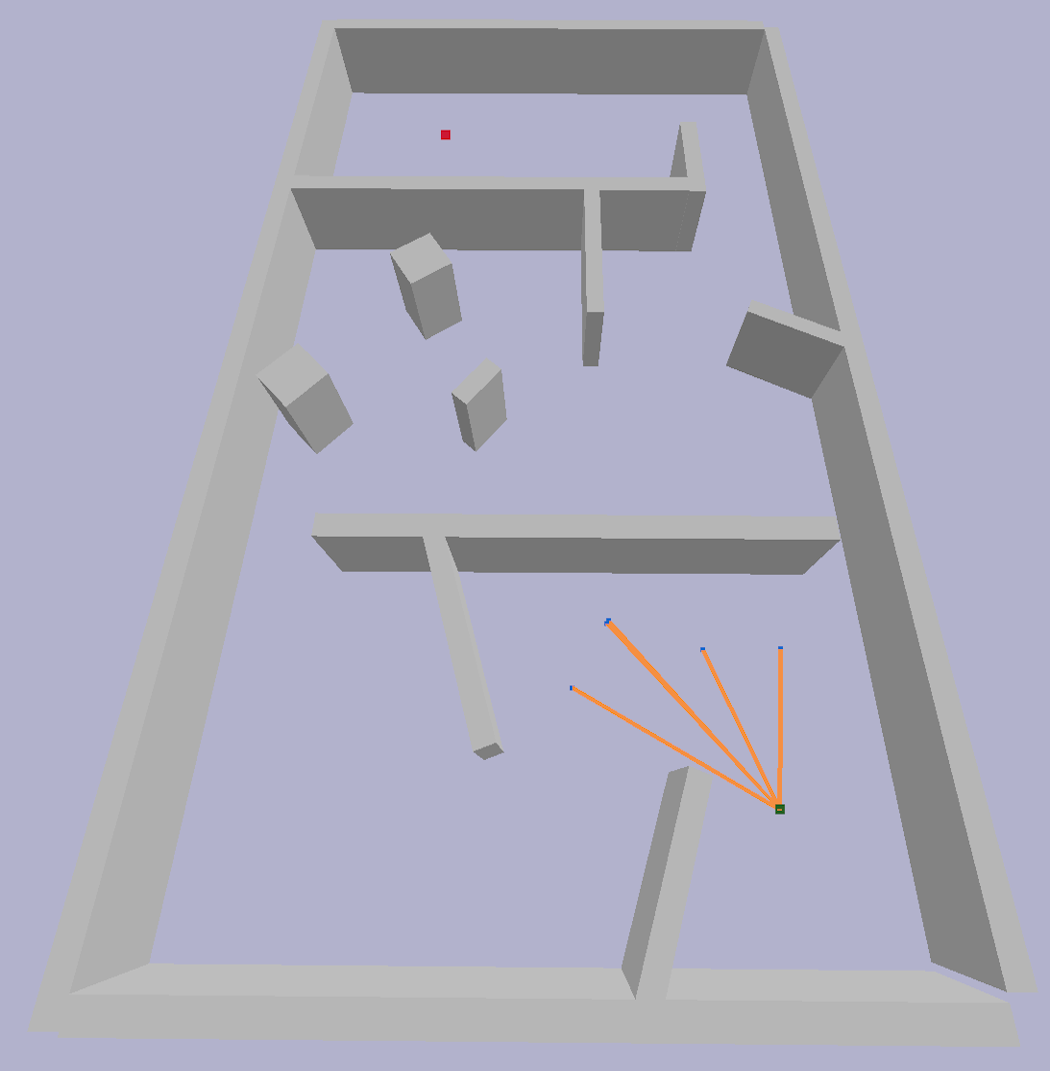
\includegraphics[width=0.4\linewidth]{figures/samp/rrtstar_unbounded.png} }}%
    \subfloat[\centering Fixed maximum local distance in \myglsentry{rrtstar}]{{\includegraphics[width=0.4\linewidth]{figures/samp/rrtstar_bounded.png} }}%
    \\
    \subfloat[\centering Maximum local distance based on space size in \myglsentry{sarrt*}]{{\includegraphics[width=0.4\linewidth]{figures/samp/sarrtstar_unbounded.png} }}%
    \subfloat[\centering Fixed maximum local distance in \myglsentry{sarrt*}]{{\includegraphics[width=0.4\linewidth]{figures/samp/sarrtstar_bounded.png} }}%
    \caption{Snapshot after 2.000 iterations of the trees generated by: (a) the \myglsentry{rrtstar} with a maximum local trajectory length based on space size, (b) \myglsentry{rrtstar} with fixed maximum local trajectory length, (c) the \myglsentry{sarrt*} with a maximum local trajectory length based on space size, and (d) the \myglsentry{sarrt*} with fixed maximum local trajectory length for the differential drive robot (red shape).
    Note that the local trajectories (in orange) are represented as linear segments only for visualization purposes.}%
    \label{fig:unic_tree}%
\end{figure}

The standard \myglsentry{ompl} \myglsentry{rrtstar} implementation typically defines a maximum local distance based on the current state space and workspace size.
This approach can lead to excessively long trajectories, especially for large spaces when two sampled states are far apart.
These trajectories frequently fail the robust feasibility check, leading to significant computational effort spent on computing uncertainty tubes only to detect early infeasibility. 
This inefficiency, resulting from highly constrained problems, slows down tree growth.
To address this, and following the approach used in the original \myglsentry{ompl} implementation, a fixed maximum distance is introduced for local trajectories. 
This adjustment does not compromise the algorithm properties, as longer trajectories can still be formed by chaining several shorter local trajectories. 
While this approach requires more iterations to ensure adequate space coverage and cost convergence, it results in more efficient tree growth under robustness constraints, as illustrated in Figure~\ref{fig:unic_tree}.
Note that the choice of this maximum local distance is also required for the applicability of the methods proposed in Chapters~\ref{chap:NN} and~\ref{chap:sampNN}.
Consequently, throughout this thesis, a maximum local trajectory length of 1.0 (meters or seconds according to the steering method used) is also applied to the proposed \myglsentry{sarrt*} variant.

Finally, all algorithms use a time step of 0.05s for the solving the \myglsentry{odes} and to perform the robust feasibility checks, and the stopping criterion of the planners is defined by a cost convergence threshold of 5\%.

\paragraph{Results}

\begin{table*}[t]
    \centering
    \begin{tabular}{l|llll|}
    \cline{2-5}
        & \multicolumn{1}{c|}{RRT$^{*}$} & \multicolumn{1}{c|}{SARRT$^*$} & \multicolumn{1}{c|}{SST$^*$} & \multicolumn{1}{c|}{SASST$^*$} \\ \hline
    \multicolumn{1}{|c|}{Success (\%)} & \multicolumn{1}{c|}{3.3} & \multicolumn{1}{c|}{\textbf{100.0}}  & \multicolumn{1}{c|}{17.3}  &  \multicolumn{1}{c|}{\textbf{100.0}}   \\ \hline
    \multicolumn{1}{|c|}{Plan time (s)} & \multicolumn{1}{c|}{952 $\pm$ 201}   & \multicolumn{1}{c|}{4145 $\pm$ 639} & \multicolumn{1}{c|}{819 $\pm$ 155}  &   \multicolumn{1}{c|}{2148 $\pm$ 320}  \\ \hline
    \end{tabular}
    \caption{
    \label{tab:samp_unicycle}
    Average planning time and success rate (no crash) of the simulated motions planned by \myglsentry{rrtstar}, \myglsentry{sarrt*}, \myglsentry{sst*}, and \myglsentry{sasst*} over 10 plans and 30 simulations per plan.}
\end{table*}

\begin{figure} [t!]
    \centering
    \includegraphics[width=0.6\linewidth]{figures/samp/unicycle_cost_conv.png} 
    \caption{Differential drive robot application: Evolution of the sensitivity as a function of the planning time of a \myglsentry{sasst*} (green), and of \myglsentry{sarrt*} (red).}%
    \label{fig:samp_unic_time}%
\end{figure}

\begin{figure} [t!]
    \centering
    \includegraphics[width=0.9\linewidth]{figures/samp/non_robust_unic.png}
    \includegraphics[width=0.9\linewidth]{figures/samp/robust_unic.png}
    \caption{Differential drive robot application: Planned trajectory (black) produced by the \myglsentry{rrtstar} (top) and the \myglsentry{sarrt*} (bottom). 
    Simulated trajectories under uncertainty are displayed in green in the case of success, and in red in the case of a crash.}%
    \label{fig:robust_unic}%
\end{figure}

Table~\ref{tab:samp_unicycle} presents comparative results averaged for each planner across 10 trajectories planned in the environment shown in Figure~\ref{fig:robust_unic}. 
Each of these 10 plans was simulated 30 times with varying values for the uncertain parameters.
The perturbations are uniformly sampled within an ellipsoid with semi-axis defined by $\delta \p$ as explained in Section~\ref{sec:tubes}.
A success is defined as a successful simulation of a plan where no collisions or control input saturations occur, despite the presence of uncertainties.

First, note that \myglsentry{sarrt*}, and \myglsentry{sasst*} variants have a robustness of 100\% compared to their respective standard, non-robust implementations.
This robustness is also illustrated in Figure~\ref{fig:robust_unic}, where the vanilla \myglsentry{rrtstar} is able to find the shortest solution which passes through a narrow corridor, however, this solution is not robust to the presence of uncertain parameters, leading to a poor robustness when executed by the controller.
On the other hand, the \myglsentry{sarrt*}, is able to find the shortest trajectory under robust constraints, leading to a 100\% success rate.
It is important to note that this success rate is assessed based on both robust collision avoidance and robust control inputs saturation.

However, this robustness comes at the cost of computational efficiency, as highlighted by the significantly higher planning times of the two robust sensitivity-aware variants when compared to their standard counterparts that focus on optimizing trajectory length.
The computational overhead is due to the time spent solving the \myglsentry{odes}, as depicted in Figure~\ref{fig:profiling_unic}, where the \emph{CC} procedure refers to either standard collision checking or the robust feasibility check, \emph{Cost} represents the trajectory cost computation, \emph{NN} stands for the nearest neighbor search, \emph{Sampling} and \emph{Steer} refer to state space sampling and local trajectory planning, respectively, \emph{Tree} handles data structure management (e.g., pruning, updating child costs, etc.), and \emph{ODEs} corresponds to the system dynamics and tubes computations.
It is show that \myglsentry{sarrt*} and \myglsentry{sasst*}, which rely on sensitivity computation, dedicate about 80\% of their total computing time to solving the \myglsentry{odes}.
This result aligns with the findings of~\cite{cTognon}, which demonstrated that, in a control-aware context, the majority of a planner computing time is taken by the closed-loop system simulation.
However, in this context, the impact is even more significant due to the additional complexity introduced by the tube computation.
Nevertheless, it is worth noting that the \myglsentry{sasst*} is much faster than the \myglsentry{sarrt*} variant as illustrated in Table~\ref{tab:samp_unicycle} and in Figure~\ref{fig:samp_unic_time} that show how the \myglsentry{sasst*} is able to converge faster than \myglsentry{sarrt*}, demonstrating that reducing the frequency of \myglsentry{odes} leads to a lower planning time.
Furthermore, the results in Figure~\ref{fig:unic_tree} strongly suggest that by incorporating uncertainty tubes, the problem becomes more constrained, requiring more iterations for the planners to converge to lower-cost regions in the state space.

\begin{figure} [t!]
    \centering
    \includesvg[width=0.8\linewidth]{figures/samp/profiling_unic.svg} 
    \caption{Differential drive robot application: Profiling of vanilla planners and robust \myglsentry{samp} variants, illustrating the contributions of various procedures to the total planning time over 1.000 iterations.}%
    \label{fig:profiling_unic}%
\end{figure}

\subsubsection{Quadrotor robot}\label{sec:quad_setup_samp}

\paragraph{Robot setup}

To further evaluate the effectiveness of the \myglsentry{samp} variants, the quadrotor model described in Section~\ref{sec:quad_model} is used with the following set of uncertain parameters: $\p = [k_{f}, \, k_{\tau}, \, x_{cx}, \, x_{cy}]$, where $k_{f}$ and $k_{\tau}$ are coefficients associated with the dynamics of the propellers, and $x_{cx}$ and $x_{cy}$ are the location of the \myglsentry{com} in the $x$-axis and $y$-axis of the quadrotor body frame, which may be uncertain due to the presence of on-board sensors for example.
The values of this vector considered in the simulations are either $\delta\p = [25\%, \, 25\%, \, 10cm, \, 10cm]$, where the first two components are a percentage of their associated nominal values. 
Therefore, in this quadrotor application, $\bPi \in \mathbb{R}^{13\times4}$, and $\bTheta \in \mathbb{R}^{4\times4}$.
As a result, the computations necessary to find the uncertainty tubes involve solving 68 \myglsentry{odes}.
The uncertainty tubes considered for this application are defined as $\Rq = [r_x, \, r_y, \, r_z]^T \in \mathbb{R}^3$, representing the uncertainty tubes along the \{x,y,z\}-axes of the state respectively, and $\Ru = [r_{u1}, \, r_{u2}, \, r_{u3}, \, r_{u4}]^T \in \mathbb{R}^4$, representing the uncertainty tubes along the four control input space axes.
Finally, the controller gains are set to $\boldsymbol{k}_{x} = [20.0, \, 20.0, \, 25.0]^T$, $\boldsymbol{k}_{v}= [9.0, \, 9.0, \, 12.0]^T$, $\boldsymbol{k}_{R}=[4.6, \, 4.6, \, 0.8]^T$, and $\boldsymbol{k}_{\omega}=[0.5, \, 0.5, \, 0.08]^T$, and the control inputs limits are set to $\u_{max} = [10.000, \, 10.000, \, 10.000, \, 10.000]^T$, corresponding to the maximum squared rotor speed expressed in (rad.s$^{-1})^2$.

\paragraph{Planning setup}

Recall that the local planning method used for the quadrotor is the kinosplines trajectory planner (see Section~\ref{sec:kinosplines}), with the following kinodynamic constraints enforced on the generated splines $[v_{max}, a_{max}, j_{max}, s_{max}] = [5.0 \, m.s^{-1}, \allowbreak 1.5 \, m.s^{-2}, \allowbreak 15.0 \, m.s^{-3}, \allowbreak 30.0 \, m.s^{-4}]$. 
Note that, again, instead of using the cost-to-go as distance metric, an efficient state-space quasi-metric is employed as defined in~\cite{cKino}.

The planning environment, referred to as the 2-Ways, is illustrated in Figure~\ref{fig:robust_quad}. 
In this setup, the drone is constrained to operate within a 2D plane by restricting the sampling to that plane.

The hyperparameters for \myglsentry{sasst*} are selected based on the recommendations in~\cite{cSST} for a quadrotor, with the following values: $N_0 = 10000$, $\delta_s = 3$, $\delta_{BN} = 5$, and $\xi = 0.9$.
The maximum trajectory length is set to 1.0s.

Finally, all algorithms use a time step of 0.05s for the solving the \myglsentry{odes} and to perform the robust feasibility checks, and the algorithms stopping criterion is defined by a cost convergence threshold of 5\%.

\paragraph{Results}

\begin{table*}[t]
    \centering
    \begin{tabular}{l|llll|}
    \cline{2-5}
        & \multicolumn{1}{c|}{RRT$^{*}$} & \multicolumn{1}{c|}{SARRT$^*$} & \multicolumn{1}{c|}{SST$^*$} & \multicolumn{1}{c|}{SASST$^*$} \\ \hline
    \multicolumn{1}{|c|}{Success (\%)} & \multicolumn{1}{c|}{61.2} & \multicolumn{1}{c|}{\textbf{100.0}}  & \multicolumn{1}{c|}{58.5}  &  \multicolumn{1}{c|}{\textbf{100.0}}   \\ \hline
    \multicolumn{1}{|c|}{Plan time (s)} & \multicolumn{1}{c|}{2801 $\pm$ 427}   & \multicolumn{1}{c|}{43451} & \multicolumn{1}{c|}{2513 $\pm$ 378}  &   \multicolumn{1}{c|}{23194}  \\ \hline
    \end{tabular}
    \caption{
    \label{tab:samp_quad}
    Average planning time and success rate (no crash) of the simulated motions planned over 10 plans for the \myglsentry{rrtstar} and \myglsentry{sst*}, and 3 trajectories only for the \myglsentry{sarrt*} and \myglsentry{sasst*} due to very high planning time.
    30 simulations with uncertain parameters where conducted for each plan.}
\end{table*}

\begin{figure} [t!]
    \centering
    \includesvg[width=0.6\linewidth]{figures/samp/sensi_cost_quad.svg} 
    \caption{Quadrotor application: Evolution of the sensitivity as a function of the planning time of a \myglsentry{sasst*} (green), and of \myglsentry{sarrt*} (red).}%
    \label{fig:samp_quad_time}%
\end{figure}

\begin{figure} [h!]
    \centering
    \includegraphics[width=0.8\linewidth]{figures/samp/non_robust_quad.png}
    \includegraphics[width=0.8\linewidth]{figures/samp/robust_quad.png}
    \caption{Quadrotor application: Planned trajectory (black) produced by the \myglsentry{rrtstar} (top) and the \myglsentry{sarrt*} (bottom). 
    Simulated trajectories under uncertainty are displayed in green in the case of success, and in red in the case of a crash.
    Note that explicitly considering the uncertainty tubes during planning does not allow the \myglsentry{sarrt*} to pass through the narrow passage.
    Additionally, it is important to note that the display tubes are augmented by the drone wingspan.}%
    \label{fig:robust_quad}%
\end{figure}

Table~\ref{tab:samp_quad} shows comparative results averaged for each planner over 10 plans for the \myglsentry{rrtstar} and \myglsentry{sst*}, and 3 trajectories only for the \myglsentry{sarrt*} and \myglsentry{sasst*} due to very high planning time, and 30 simulations with uncertain parameters. 
The perturbations are uniformly sampled within an ellipsoid with semi-axis defined by $\delta \p$ as explained in Section~\ref{sec:tubes}.
First, it is important to note robust efficiency of the proposed \myglsentry{samp} variants which achieve both 100\% robustness compared to their non-robust vanilla implementation, as highlighted by Figure~\ref{fig:robust_quad}.

However, as explained in Section~\ref{sec:samp}, the set of \myglsentry{odes} must be solved at each algorithm iteration, one per iteration in the case of \myglsentry{sasst*} and at least tens to hundreds of times for the \myglsentry{sarrt*}.
Although this results in high computation times for simple systems like the differential drive robot presented above, the planning time depicted in Table~\ref{tab:samp_quad} and the cost convergence rate show in Figure~\ref{fig:samp_quad_time} highlight the intractability of such optimal planning techniques for the quadrotor case, which involve solving hundreds of \myglsentry{odes}.
Similar to the differential drive robot, the prohibitively long planning time is closely linked to the time spent solving the \myglsentry{odes}, as shown in Figure~\ref{fig:profiling_quad}, where the \emph{CC} procedure refers to standard collision checking or the robust feasibility check, \emph{Cost} is the trajectory cost computation procedure, \emph{NN} stands for the nearest neighbor search, \emph{Sampling} and \emph{Steer} refer to the state space sampling and local trajectory planning respectively, \emph{Tree} procedure is in charge of the data structure management (e.g. pruning, child cost update, etc.), and finally \emph{ODEs} stands for the sensitivity and tubes computations.
Therefore, the frequency of \myglsentry{odes} solving must be further reduced, as even the \myglsentry{sasst*}, which performs only a single computation per iteration, faces challenges due to the tens of thousands of iterations required to adequately explore the space.

\begin{figure} [t!]
    \centering
    \includesvg[width=0.8\linewidth]{figures/samp/profiling_quad.svg} 
    \caption{Quadrotor application: Profiling of vanilla planners and robust variants, illustrating the contributions of various procedures to the total planning time over 1.000 iterations.
    }%
    \label{fig:profiling_quad}%
\end{figure}

\subsubsection{Conclusions}

The proposed \myglsentry{samp} variants enable the generation of robust trajectories that account for parametric uncertainties for both differential drive and quadrotor robots, outperforming their standard non-robust counterparts in terms of robustness w.r.t. uncertain parameters.
However, simulating the systems closed-loop dynamics and computing the tubes at each tree extension is computationally demanding, as highlighted by the very high planning time of the \myglsentry{samp} variants and mentioned in~\cite{cTognon}.
Although the \myglsentry{sst*} requires more iterations to achieve convergence compared to \myglsentry{rrtstar} as shown in~\cite{cSST}, its approach of computing uncertainty tubes only once per iteration results in improved planning times for \myglsentry{sasst*} compared to \myglsentry{sarrt*}.
Therefore, the following section presents a decoupled approach to further reduce the frequency of simulating the closed-loop dynamics and computations of the subsequent uncertainty tubes.

\section{Decoupled approach}\label{sec:decoupled}

As illustrated in Section~\ref{sec:samp_simu}, the proposed \myglsentry{samp} variants are efficient for simple systems but, they face challenges with more complex ones, such as the quadrotor. 
Achieving effective state-space coverage and convergence to an optimal solution w.r.t. sensitivity-based cost requires thousands of iterations, each involving the resolution of many \myglsentry{odes}. 
This creates a bottleneck for the method, particularly when solving the \myglsentry{odes} requires tens of milliseconds for hundreds of time steps, as common for complex systems.
Therefore, this section introduces a decoupled approach that first plans a (near) time-optimal trajectory and optimizes its sensitivity in a second stage.
This method minimizes the frequency of solving the \myglsentry{odes}, offering a more efficient algorithm for complex systems, such as quadrotor, to generate robust trajectories with near-optimal sensitivity.

Since the cost function of Equation~(\ref{eq:cost_function}) corresponds to the integration of the sensitivity over the trajectory, starting with an initial (near) time-optimal trajectory is a reasonable strategy for generating initial solutions of relatively high quality (i.e. near the optimal solution) w.r.t. the sensitivity cost.
The proposed decoupled approach is based on a lazy sensitivity-aware variant, referred to as \gls{lazysamp}, that first plans a robust (near) time-optimal trajectory.
This trajectory is then locally optimized for minimizing the cost function~(\ref{eq:cost_function}) via a robust variant of the ``shortcut'' technique classically used to smooth solutions of randomized planners~\cite{cShortcut}. 

The following section introduces a lazy robust checking strategy. 
Although Section~\ref{sec:samp_simu} demonstrates that \myglsentry{sst*} achieves faster convergence, this lazy approach cannot be applied to \myglsentry{sst*}. 
\myglsentry{sst*} depends on immediate collision verification and aggressive pruning to maintain a sparse and optimal tree structure. 
It requires prompt evaluation of node quality and trajectory costs to retain only the most promising nodes.
Delaying collision checks, as in the lazy approach, would compromise the \myglsentry{sst*} ability to efficiently prune suboptimal nodes and update its witness set dynamically, potentially resulting in an inefficient and cluttered tree. 
Consequently, the lazy robust checking strategy outlined in the next subsection is implemented within \myglsentry{rrtstar}.

\subsection{Global robust motion planning with lazy strategy (LazySARRT*)}\label{sec:lazy_rrt*}

This subsection present the \gls{lazysarrt*}, as a particular instance of \myglsentry{lazysamp}, that plans a robust (near) time-optimal trajectory.
The algorithm not only provides a (near) time-optimal trajectory but also ensures that the resulting trajectory is robustly feasible w.r.t. the state uncertainties and also that control inputs remain in their allowed bounds.
However, as highlighted in Section~\ref{sec:samp}, the number of \myglsentry{odes} computation within the \myglsentry{rrtstar} must remain as limited as possible to avoid a too long computing time. 
For this reason, trajectory robustness is checked in a lazy way, only when a better solution is found, and reconnecting the nodes optimally w.r.t. the trajectory time if necessary.
The lazy process is inspired from ideas in~\cite{cLazy1,cLazy2}, with the addition of maintaining a set of non-robust parents ($Q_{collide}$) for each node.
Consequently, unlike the \myglsentry{samp} methods described in Section~\ref{sec:samp}, the tree built by the lazy variant is not inherently robust; only the final solution is robust.

\begin{algorithm}[h!]
    \caption{LazySARRT$^* [q^{init}, q^{goal}]$}\label{alg:LazySARRT*}
    \begin{algorithmic}[1]
        \State $T \gets$ InitTree$({q^{init}, q^{goal}});$
        \While{\textbf{not} StopCondition$(T, {q^{goal}})$}  
            \State $q^{rand} \gets $Sample()$;$
            \State $q^{nearest} \gets$ Nearest$(T,{q^{rand}});$
            \State Extend$(T, q^{rand}, q^{nearest});$
            \State $Q_{sol} \gets$ CheckForSolution$(T, q^{init}, q^{goal});$
            \If{$Q_{sol} \neq \emptyset$}
                \For { i = 0 and  i < size($Q_{sol}$)-1}
                    \State $S_0 \gets $GetNodeConditions$(Q_{sol}^{i});$
                    \State $\q_d \gets $Steer$(Q_{sol}^{i}, Q_{sol}^{i+1});$
                    \State $\left \{\q_n, \u_n, \Rq, \Ru, S_F \right \}  \gets $SolveODEs$(\q_d, S_0);$
                    \If {\textbf{not} IsRobust$(\Rq,\Ru, \q_n, \u_n)$}
                        \State $T \gets $RobustReconnect$(T, Q_{sol}^{i});$
                    \EndIf
                \EndFor
            \EndIf
        \EndWhile
        \State \textbf{return} GetTrajectory$(T, q^{init}, q^{goal})$;
    \end{algorithmic}
\end{algorithm}

\begin{figure} [h!]
    \centering
    \includegraphics[width=0.8\linewidth]{figures/samp/lazyrrtstar.png} 
    \caption{Illustration of the \myglsentry{lazysarrt*} process.
    When a solution is found (red), the uncertainty tubes (green) are computed and used for robust collision checking.
    In the case of a collision with the tubes, the tree is disconnected at the first edge found to be in collision and then optimally reconnected (indicated by blue edges) while considering previous non-robust attempts. 
    Specifically, in this case, $q^{col}$ cannot be reconnected to its parent during subsequent tree expansion phases.
    }%
    \label{fig:lazysarrt*}%
\end{figure}

Algorithm~\ref{alg:LazySARRT*} provides the pseudo-code of the \myglsentry{lazysarrt*} algorithm.
The first stage applies the standard \myglsentry{rrtstar} (line 1-5) where the Extend procedure performs the standard collision checking (i.e. without uncertainty tubes), optimal connection, and rewiring phase for the given sample  $q^{rand}$ as in~\cite{cRRTstar}.
The algorithm then verifies at each iteration whether a new, lower-cost solution has been discovered. 
If a better solution is identified, the set of nodes $Q_{sol}$, which enables the reconstruction of this solution, is retrieved (line 6).

Next, for each local trajectories between two consecutive nodes in this set, the \myglsentry{odes} are solved, and the uncertainty tubes computed (line 9-11).
The algorithm then verifies the robust feasibility of the local trajectory using a robustness test (see Appendix~\ref{chap:appendixA}) w.r.t. obstacles but also control inputs saturation. 
If a local trajectory is found to be non-robustly feasible, all nodes in the tree connected to $Q_{sol}^i$ are disconnected and reconnected using the RobustReconnect procedure explain below (line 13).

The RobustReconnect procedure may differ depending on the specific \myglsentry{lazysamp} variant used (see Chapter~\ref{chap:sampNN}). 
In the case of \myglsentry{lazysarrt*}, where maintaining an optimal tree is required, it is illustrated by Figure~\ref{fig:lazysarrt*} and operates as follows:
\begin{itemize}
    \item For all tree nodes, a set of non-robust parents $Q_{collide}$ is maintained. 
    The RobustReconnect procedure starts by adding $Q_{sol}^i$ in the set of non-robust parents of $Q_{sol}^{i+1}$ (i.e., $Q_{sol}^i$ will no longer be considered as a potential parent for the node $Q_{sol}^{i+1}$).
    \item Then, all the nodes of the tree from $Q_{sol}^i$ are disconnected and, for each of them, the vanilla Extend procedure is executed considering their associated $Q_{collide}$ set.
    As in the standard \myglsentry{rrtstar}, an optimal re-connection phase is first attempted.
    All nodes must be evaluated for optimal reconnection, as the non-robust invalid edge may be reconnected, but its children nodes could potentially find improved connections.
    \item If no re-connection is found for a node, then the node is deleted from the tree. 
    Otherwise, the rewiring phase is carried out considering the $Q_{collide}$ set.
\end{itemize}

The output of \myglsentry{lazysarrt*} is a (near) time-optimal trajectory that is feasible in terms of both collision avoidance and actuator saturation, accounting for uncertainties.
It is however not optimized in terms of the sensitivity. 
Therefore, its robustness can be further improved.

\subsection{Local robust sensitivity optimization}

\begin{algorithm}[htp]
    \caption{SAShortcut [$\q_{d,SARRT^*}$]}\label{alg:SAshortcut}
    \begin{algorithmic}[1]
        \State $\{\q_{d,best}, cost_{best}\} \gets \{\q_{d,SARRT^*}, $Cost$(\q_{d,SARRT^*}) \};$
        \State $q_d^{init} \gets \q_{d,best}^0; q_d^{goal} \gets \q_{d,best}^F;$
        \While{\textbf{not} StopCondition$()$} 
            \State $\{q_d^{1}, q_d^{2}\} \gets$ SampleOnTraj$(\q_{d,best});$
            \State $\q_{d,shct} \gets $Steer$(q_d^{1}, q_d^{2});$
            \If{CollisionFree$(\q_{d,shct})$}
                \State $\q_{d,start} \gets $Steer$(q_d^{init}, q_d^{1});$
                \State $\q_{d,end} \gets $Steer$(q_d^{2}, q_d^{goal});$
                \State $\q_{d,new} \gets \q_{d,start}+\q_{d,shct}+\q_{d,end};$
                \State $S_0 \gets $GetNodeConditions$(q_d^{init});$
                \State $\{\q_n, \u_n, \Rq, \Ru, S_F\}  \gets $SolveODEs$(\q_{d,new}, S_0);$
                \State $cost_{new} \gets $Cost$(\q_{d,new});$
                \If{CostBetterThan$(cost_{new}, cost_{best})$}:   
                    \If {IsRobust$(\Rq,\Ru, \q_n, \u_n)$}
                        \State $\{\q_{d,best}, cost_{best}\} \gets \{\q_{d,new}, cost_{new}\};$
                    \EndIf
                \EndIf
            \EndIf
        \EndWhile
    \State \textbf{return} $\q_{d,best}$
    \end{algorithmic}
\end{algorithm}

In order to improve the sensitivity-based cost function, a local optimization is performed using a simple robust sensitivity-aware variant of the ``shortcut'' smoothing algorithm~\cite{cShortcut}, called \gls{SAshortcut} and described in Algorithm~\ref{alg:SAshortcut}. 
% A more detailed discussion regarding the robust sensitivity-aware local optimization can be found in Chapter~\ref{chap:sampNN}.

The algorithm is first initialized with the robust trajectory resulting from the \myglsentry{lazysarrt*} presented above (line 1).
It is important to note that the robustness of the initial trajectory is a crucial assumption, as the \myglsentry{SAshortcut} algorithm does only guarantee the generation of a robust trajectory if the initial trajectory is robust.
Nevertheless, the algorithm preserves this robustness throughout its local optimization process.
At each iteration, the algorithm randomly samples two states $\{q_d^{1}, q_d^{2}\}$, along the current best trajectory (line 4).
Next, it computes the local trajectory between the two samples $\q_{d,shct}$ (line 5).
To minimize the frequency of solving the \myglsentry{odes}, a lazy approach is employed.
First, the algorithm ensures that the proposed shortcut is collision-free (line 6). 
Unlike the classical shortcut method, which compares only the costs of the original and proposed trajectory segments, the entire trajectory is re-evaluated to incrementally compute the sensitivity cost (lines 7–12).
It is important to note that both the cost and uncertainty tubes are derived from the \myglsentry{odes}. 
Thus, to avoid redundant computations, the \myglsentry{odes} are solved before performing the cost comparison.
Finally, if the new solution has a lower sensitivity cost (line 13), then a robust feasibility check is performed before updating the trajectory portion in case of success (line 14-15).

\subsection{Simulation results}
\subsubsection{Differential drive robot}

\paragraph{Robot setup}

The robot setup is the same as the one described in Section~\ref{sec:unic_setup_samp}.

\paragraph{Planning setup}

The environment is the same as presented in Figure~\ref{fig:robust_unic}.
The \myglsentry{lazysarrt*} is performed with a cost convergence of 5\% and the \myglsentry{SAshortcut} with a cost convergence of 1\%.
The decoupled approach is compared to the \myglsentry{sasst*} as it is the fastest compared to \myglsentry{sarrt*}.
Finally, all algorithms use a time step of 0.05s for the solving the \myglsentry{odes} and to perform the robust feasibility checks.

\paragraph{Results}

The decoupled approach is tested for the same differential drive robot settings as in Section~\ref{sec:samp_simu} where the \myglsentry{lazysarrt*} produces robust (near) length-optimal trajectories.
Table~\ref{tab:lazySAMP_unic} presents the average computation times over 10 runs for \myglsentry{sasst*} and the two core procedures of the proposed decoupled approach (\myglsentry{lazysarrt*}, \myglsentry{SAshortcut}), demonstrating a time savings of only 29.56\%.
The average cost found by the decoupled approach is of $0.925 \pm 0.032$ against $0.894 \pm 0.046$ for the \myglsentry{sasst*}, denoting a sub-optimallity of $3.47\%$.

\input{figures/tables/lazySAMP_unic.tex}

\begin{figure}[t!]
    \centering
    \includegraphics[width=0.7\linewidth]{figures/samp/sensi_cost_unic.png}
    \caption{Differential drive robot application: Trajectory cost resulting of the decoupled approach over 3 runs (red, green, blue), the dashed purple cost correspond to the sensitivity-optimal reference trajectory found by the \myglsentry{sasst*}.}
    \label{fig:sensi_cost_unic}
\end{figure}

The process is illustrated by the Figure~\ref{fig:sensi_cost_unic} where it is worth noting that during the \myglsentry{lazysarrt*} planning process, trajectory length optimization leads to a reduction in sensitivity cost, even though this was not the primary objective. 
This supports the choice of a (near) length-optimal trajectory as the initial guess for \myglsentry{SAshortcut} and validates the use of a length-based metric as the state-space metric when optimizing sensitivity within the \myglsentry{sarrt*} and \myglsentry{sasst*} methods discussed in Section~\ref{sec:samp_simu}.

\subsubsection{Quadrotor robot}

\paragraph{Setup}

The quadrotor setup is the same as described in Section~\ref{sec:quad_setup_samp}.
Another set of uncertain parameters is introduced, such that in the 2-Ways environment, one set allows the robot to pass through the narrow passage, while the other does not.
The values of these vectors considered in the simulations are either $\delta\p_{low} = [10\% , 10\% ,  5cm , 5cm]$ or $\delta\p_{high} = [25\%, \, 25\%, \, 10cm, \, 10cm]$, where the first two components are a percentage of their associated nominal values. 

\paragraph{Planning}

The performances of the decoupled approach are evaluated in three different environments, also considering different parametric uncertainties.
In the 2D environments (U-shape and 2-Way), the quadrotor is forced to evolve at fix altitude by generating kinosplines only between samples within a plane and by not allowing displacements along the z-axis.
The \myglsentry{lazysarrt*} is performed with a cost convergence of 5\% (i.e., the algorithm will stop optimizing the trajectory when the improvement in cost from one iteration to the next is less than 5\%) and the \myglsentry{SAshortcut} with a cost convergence of 1\%.
The decoupled approach is compared to the \myglsentry{sasst*} as it is the fastest compared to \myglsentry{sarrt*}.
Finally, all algorithms use a time step of 0.05s for the solving the \myglsentry{odes} and to perform the robust feasibility checks.

\paragraph{Results}

Table~\ref{tab:lazySAMP_quad} gathers the average computing times of \myglsentry{sasst*} and of the two core procedures of the proposed decoupled approach (\myglsentry{lazysarrt*}, \myglsentry{SAshortcut}), as well as the average final cost found by \myglsentry{sasst*} and \myglsentry{SAshortcut}. 
The mean values associated with \myglsentry{sasst*} were obtained over 3 runs (due to the very high computational time) while those associated with the proposed decoupled approach are averaged over 10 runs.

\newcolumntype{C}[1]{>{\centering\arraybackslash }b{#1}}
\begin{table*}[t!]
    \centering
    \begin{tabular}{|C{0.185\linewidth}||C{0.095\linewidth}|C{0.12\linewidth}|C{0.12\linewidth}|C{0.09\linewidth}|}
     \hline
      & U-shape & 2-Way$_{low}$ & 2-Way$_{high}$ & 3D \\
     \hline
     \hline
     Time \myglsentry{sasst*}  (s) & 7221 & 16615 & 23194 & 26875 \\
     \hline
     Time \myglsentry{lazysarrt*} (s) & \textbf{673} \quad $\pm$ 247& \textbf{2506} \quad\quad $\pm$ 305& \textbf{3271} \quad\quad $\pm$ 440& \textbf{2388} \quad $\pm$ 342\\
     \hline
     Time \myglsentry{SAshortcut} (s) & \textbf{453} \quad $\pm$ 191& \textbf{374} \quad\quad $\pm$ 173& \textbf{753} \quad\quad $\pm$ 104& \textbf{577} \quad $\pm$ 229\\
     \hline 
     Decoupled approach time gain (\%)  & 84.4 & 82.7 & 82.6 & 89.0 \\
     \hline
     \hline
      Cost \myglsentry{sasst*} & 0.317 & 0.292 & 5.127 & 0.510 \\
     \hline
      Cost decoupled approach & \textbf{0.324} \quad $\pm$ 0.003& \textbf{0.298} \quad $\pm$ 0.002& \textbf{5.274} \quad\quad $\pm$ 0.041& \textbf{0.523} \quad $\pm$ 0.071\\
     \hline
      Sub-optimality decoupled approach (\%) & 2.21 & 2.01 & 2.87 & 2.55 \\
     \hline
    \end{tabular}
    \caption{
    \label{tab:lazySAMP_quad}
    Quadrotor application: Average values of costs and computing times for the different methods in several environments.
    Standard deviations are provided for the SAMP results only as the SST$^*$ results do not contain enough runs.
    }
\end{table*}

\begin{figure}[h!]
    \centering
    \subfloat[\centering ]{{\includegraphics[width=0.45\linewidth]{figures/samp/U_shape_3in1_before.png} }}%
    \subfloat[\centering ]{{\includegraphics[width=0.45\linewidth]{figures/samp/U_shape_3in1_after.png} }}%
    \\
    \includegraphics[width=0.7\linewidth]{figures/samp/U_shape_3in1_sensi.png}
    \caption{Quadrotor application: Three trajectories (red, green, blue) produced by \myglsentry{lazysarrt*} (a), and the three trajectories resulting from \myglsentry{SAshortcut} (b), with the evolution of their respective sensitivity (bottom). 
    The dashed black trajectory (a, b) and the dashed purple cost (bottom) correspond to the sensitivity-optimal reference trajectory found by the \myglsentry{sasst*}.}
    \label{fig:U_shape}
\end{figure}

\begin{figure} [t!]
    \centering
    \subfloat[\centering ]{{\includegraphics[width=0.4\linewidth]{figures/samp/2Ways_low_3in1_before.png} }}%
    \subfloat[\centering ]{{\includegraphics[width=0.4\linewidth]{figures/samp/2Ways_low_3in1_after.png} }}%
    \\
    \subfloat[\centering ]{{\includegraphics[width=0.4\linewidth]{figures/samp/2Ways_high_3in1_before.png} }}%
    \subfloat[\centering ]{{\includegraphics[width=0.4\linewidth]{figures/samp/2Ways_high_3in1_after.png} }}%
    \caption{Quadrotor application: Trajectories planned by: (a) the \myglsentry{lazysarrt*} with low parameter uncertainties, (b) after the \myglsentry{SAshortcut} with low parameter uncertainties, (c) the \myglsentry{lazysarrt*} with high parameter uncertainties, and (d) after the \myglsentry{SAshortcut} with high parameter uncertainties.
    Note that one (near) sensitivity-optimal trajectory planned by the \myglsentry{sasst*} is displayed in dashed black.}%
    \label{fig:2way}%
\end{figure}

\begin{figure}[h!]
    \centering
    \includegraphics[width=0.58\linewidth]{figures/samp/3D_full_view.png}
    \includegraphics[width=0.58\linewidth]{figures/samp/3D_ZYprofile.png}
    \includegraphics[width=0.58\linewidth]{figures/samp/3D_sensi.png}
    \caption{Quadrotor application: Trajectories produced by \myglsentry{lazysarrt*} (green), \myglsentry{SAshortcut} (red), and \myglsentry{sasst*} (dashed black) in a 3D environment (top). 
    A profile view along the YZ plane is given (middle) as well as the evolution of the sensitivity (red) and the optimal one found by the \myglsentry{sasst*} (dashed blue) (bottom).}
    \label{fig:3D}
\end{figure}

\paragraph{2D U-Shape Environment} 

Figure~\ref{fig:U_shape} shows how the decoupled approach is able to produce solutions that mimic the optimal one found by the \myglsentry{sasst*} in the so called U-shape environment considering the $\delta\p_{low}$ parametric uncertainty vector.
Furthermore, according to the results shown in Table~\ref{tab:lazySAMP_quad} and in Figure~\ref{fig:U_shape}, \myglsentry{SAshortcut} produces solutions with sensitivity costs close to the optimal reference found by \myglsentry{sasst*}. 
Also note the huge time saving (6.4 time faster) of the proposed method compared to the \myglsentry{sasst*}.
Additionally, it is again worth to note that during the \myglsentry{lazysarrt*} planning, trajectory length optimization results in a reduction of the sensitivity cost, further corroborating the observations made in the differential drive robot application.

Finally, note that the average computing time of \myglsentry{lazysarrt*} in this case is low compared to the other environments. 
This is mainly due to the fact that in this case the time-optimal trajectory is far from the obstacles and therefore few re-connections via the \myglsentry{lazysarrt*} RobustReconnect procedure are performed when extending the tree.

% \begin{figure}[H]
%     \centering
%     \includegraphics[width=0.7\linewidth]{figures/samp/U_shape_3in1_before.png}
%     \includegraphics[width=0.7\linewidth]{figures/samp/U_shape_3in1_after.png}
%     \includegraphics[width=0.7\linewidth]{figures/samp/U_shape_3in1_sensi.png}
%     \caption{Three trajectories (red, green, blue) produced by \myglsentry{lazysarrt*} (top), and the three trajectories resulting from \myglsentry{SAshortcut} (middle), with the evolution of their respective sensitivity (bottom). 
%     The dashed black trajectory (top, middle) and the dashed purple cost (bottom) correspond to the sensitivity-optimal reference trajectory found by the \myglsentry{sasst*}.}
%     \label{fig:U_shape}
% \end{figure}

\paragraph{2D 2-way Environment} 

% \begin{figure}[htp]
%     \centering
%     \includegraphics[width=0.7\linewidth]{figures/samp/Contribution-example1.png}
%     \includegraphics[width=0.7\linewidth]{figures/samp/Contribution-example2.png}
%     \caption{Solutions with their uncertainty tube (in green) computed by the decoupled approach between the same start/goal states of a quadrotor dynamical model for small/high parameters uncertainties (top/bottom, respectively)}
%     \label{fig:2way}
% \end{figure}

This environment referred to Figure~\ref{fig:2way} where the two sets of uncertainties $\delta\p_{low}$ and $\delta\p_{high}$ are considered.

As shown in Figure~\ref{fig:2way}, in the presence of small uncertainties the decoupled approach produces a trajectory allowing to use the narrow passage. 
However, while considering large uncertainties, the non-robust time optimal trajectory, which goes through the narrow passage, cannot be taken as a collision is found by considering the uncertainty tube as shown in red in the Figure~\ref{fig:2way}.
Nevertheless, the approach is able to find the fastest trajectory apart from those passing through this passage.

In both cases the average cost of the solutions produced by the decoupled approach is close to that found by \myglsentry{sasst*} as shown in Table~\ref{tab:lazySAMP_quad}, where 2-Way$_{low}$ refers to the presence of small uncertainties and 2-Way$_{high}$ to the presence of large uncertainties.
The average computing time of the \myglsentry{sasst*} is equivalent in both cases as it is performed on exactly the same environment.
However, note that the average computing time of the \myglsentry{lazysarrt*} is longer than in the U-shape case because the time-optimal trajectories must pass through a location where many collisions may occur. 
Moreover, in the 2-Way$_{high}$ case the \myglsentry{lazysarrt*} computing time is longer than in the 2-Way$_{low}$ as even more non-robust trajectories are found.
This is because more iterations are needed before considering a neighborhood without nodes passing through the narrow corridor.
Finally, one can note that the \myglsentry{SAshortcut} computing time remains of the same order of magnitude for both cases as that of the U-shape, and again the decoupled approach produces a solution much faster (5.7 time faster) than \myglsentry{sasst*}.

\paragraph{3D Environment} 

The uncertainty set considered in this full 3D environment is $\delta\p_{low}$.
As shown in Figure~\ref{fig:3D}, once again the decoupled approach produces trajectories that mimic the optimal obtained by the \myglsentry{sasst*}.
It is interesting to note the impact of the \myglsentry{SAshortcut} procedure on the z component in addition to the impact on the \{x,y\} components already seen in the previous 2D environments.
The average computing time of the shortcut is similar to other environments according to Table~\ref{tab:lazySAMP_quad}.
Again, the proposed method produces a near-optimal trajectory much faster (9 time faster) than conventional optimal planners.

Finally, it is worth noting that in all cases, the significantly higher planning time of the \myglsentry{sasst*} compared to the lazy approach indicates that robust planning in a constrained environment requires a greater number of iterations to achieve adequate state-space coverage and converge effectively.
Furthermore, the significantly greater time gains observed in the quadrotor application compared to the differential drive robot application indicate that minimizing the number of times the \myglsentry{odes} need to be solved by the planner for more complex systems is crucial for keeping computation times manageable when planning with sensitivity.

\section{Conclusions}\label{sec:concl}

This chapter presented the general methodology for generating robust, sensitivity-aware variants, referred to as \myglsentry{samp}. 
To address the challenge of robust sensitivity-optimal trajectory generation, two variants—\gls{sarrt*} and \gls{sasst*}—were introduced. 
While these methods were demonstrated to be effective for simpler systems, such as differential drive robots, they result in high computation times. 
For more complex systems, such as quadrotors, their direct application becomes computationally unmanageable.
This limitation is primarily due to the significant time required to solve the \myglsentry{odes}.

To overcome this bottleneck, a decoupled framework was specifically designed to manage global planning using sensitivity-based metrics more efficiently than traditional asymptotically optimal sampling-based tree planners. 
This chapter introduced the \gls{lazysamp} variants, which aim to reduce the frequency of solving the \myglsentry{odes}. 
Simulations demonstrated that while the decoupled approach yields near sensitivity-optimal trajectories with moderate time savings for simpler systems like differential drive robots, it achieves substantial time savings as system complexity increases.

However, computing time remain affected by the need to solve the \myglsentry{odes}, as the associated computational cost scales approximately linearly with their number.
Additionally, the decoupled approach generates trees that are not inherently robust; only the final trajectory satisfies robustness requirements, limiting the reusability of the generated plans for tasks such as re-planning.

To address these challenges, the next chapters of this thesis will explore learning techniques to accelerate \myglsentry{odes} computation and propose motion planning algorithms that leverage these learned models.